\section{Part A}
%=========================Default Triangles====================================%
\subsection{Rate Vs. Fill Rate:}
The objective of first experiment is to find the crossover point for the unlit untexture triangles between the fill rate and geometry rate. This is done by testing both rates for different triangle sizes. The results are shown in Figure \ref{fig:fill_geo1}(a) on a log-log scale, where the fill rate (MFrags/Sec) increases as expected for small triangles and geometry rate (MVerts/Sec) decreases. The crossover point is between triangle area between 2 and 4 pixels. We notice that for triangle of size between 2 to 16 pixels the geometry rate is almost constant.  Even though the geometry rate is the highest but this could be due to more efficient use of caching. Since the triangles are of small size, and due to spatial locality, more triangle can be fetched and put into the cache. On the other side, the rapid change on the fill rate starts to slow down at triangle size greater than 16 pixels. This could be due to the fact the geometry stage is not sending enough work for the rasterization stage. So even the overall fill rate increases as the triangle size increases, but the slope of the line is not the same overall.

\begin{figure}[!tbh]
 \centering  
 \subfloat[Default]
    {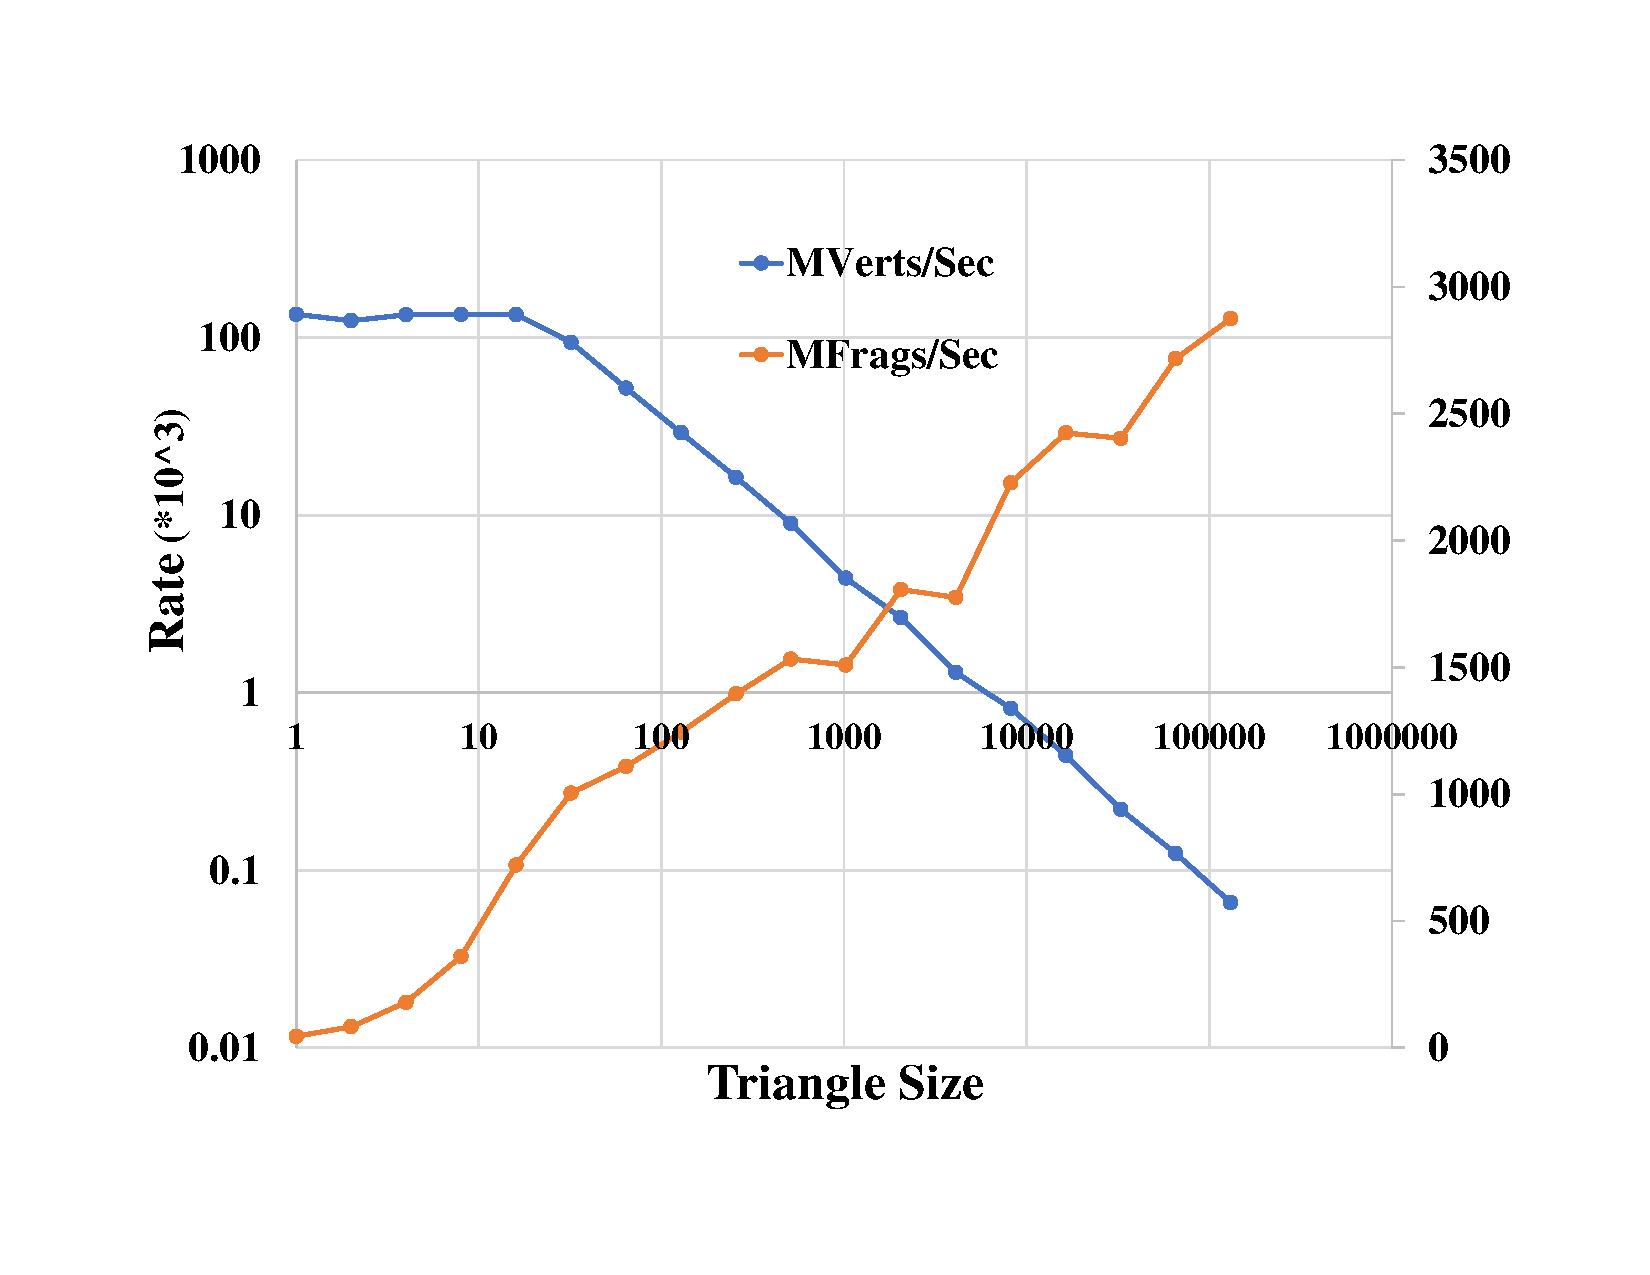
\includegraphics[width=0.49\linewidth]{fig/fill_geo.pdf}}   
 \subfloat[Lit Triangles]
   {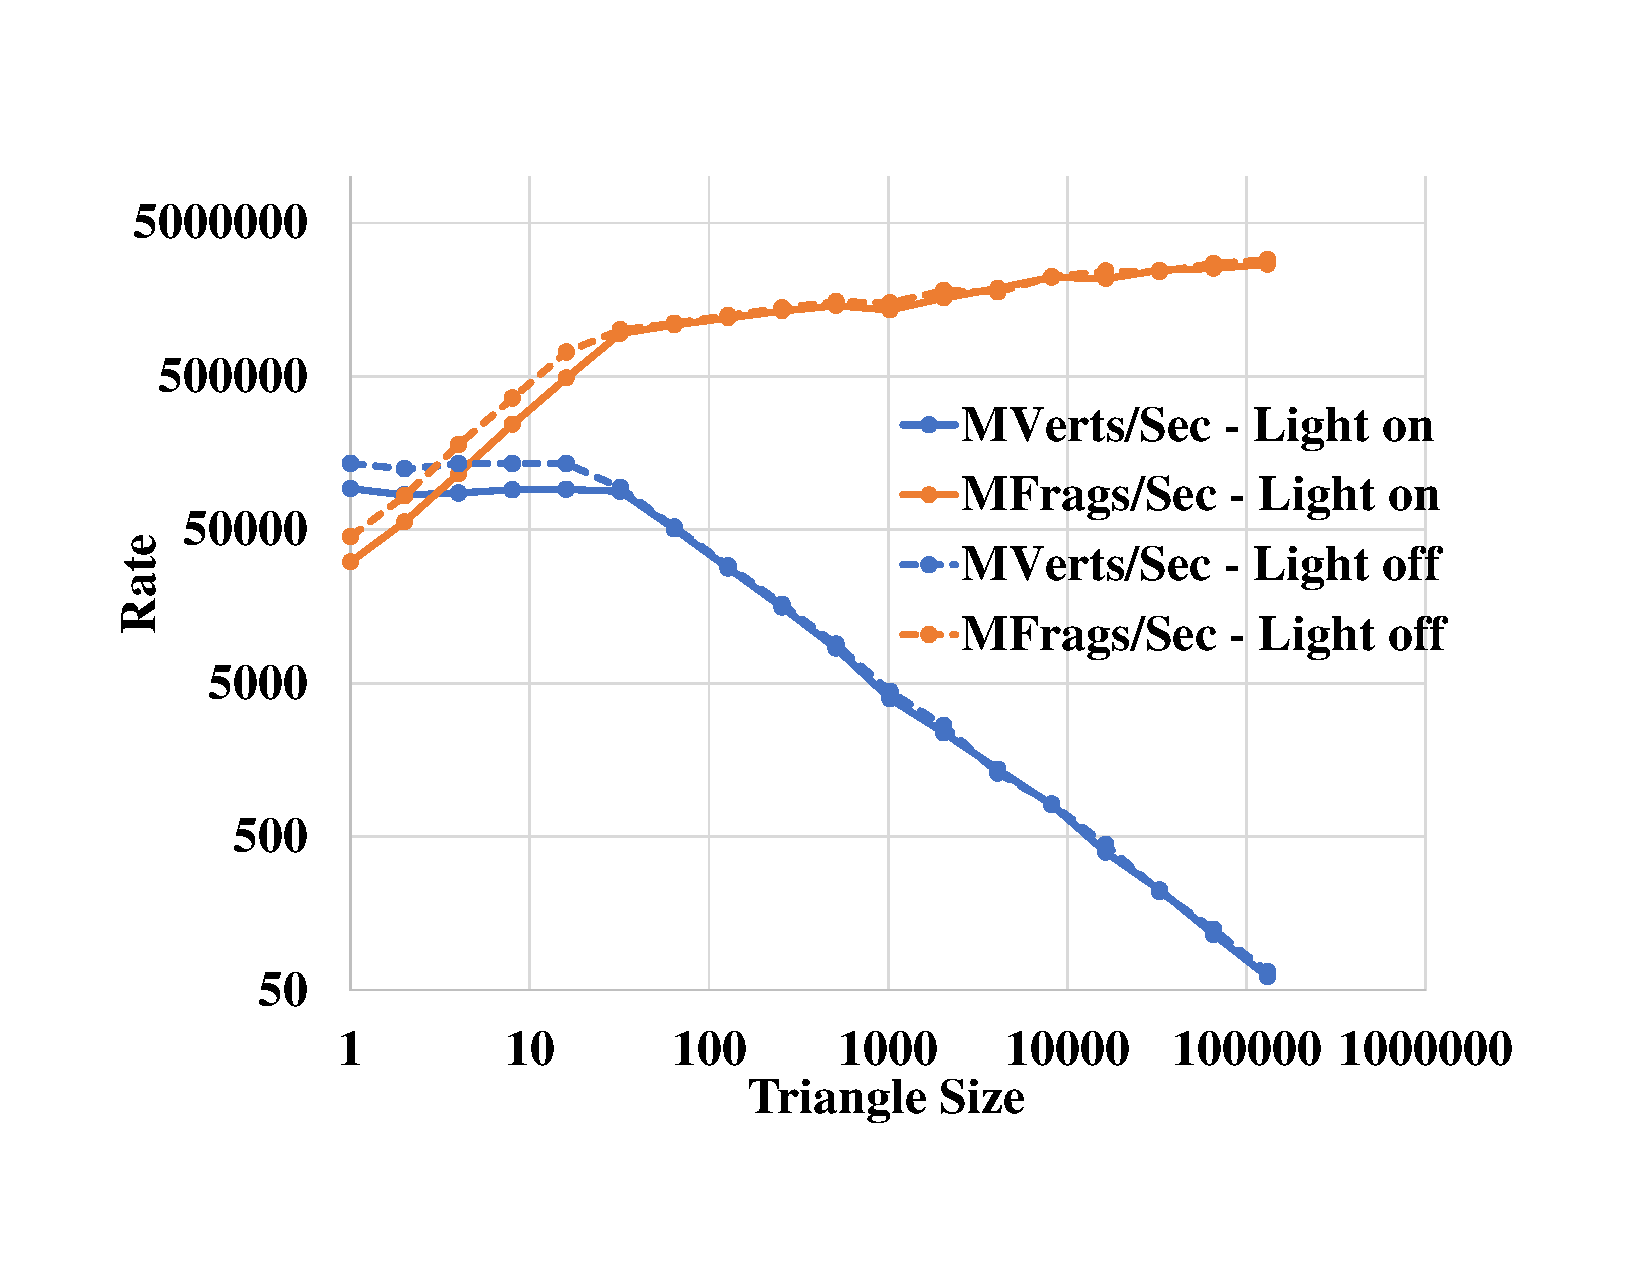
\includegraphics[width=0.49\linewidth]{fig/fill_geo_lit.pdf}}
  \caption{millions of vertices and millions of fragments}
   \label{fig:fill_geo1}
\end{figure} 

%========================= Lit Triangles ====================================%
\subsection{Geometry Rate Vs. Fill Rate on Lit Triangles:}\label{sec:lit}
The previous test was done on unlit, untexture triangles which was the default setting. Now we turn on the light on the triangles and do the same test and compare the results with the unlit triangles. The results are shown in Figure \ref{fig:fill_geo1}(b) where the crossover point is almost the same (between triangle size of 2 and 4 pixels). Additionally, we notice that the upper portion of the graph (towards triangle of size greater than 32 pixels) is identical i.e., the dotted and the solid lines overlaps for fill and geometry rates. For the lower part of the graph, it is understood that the geometry will decrease since the lighting is being processed at this stage and thus more work need to done for computing each vertex. This will directly affect the fill rate since less work is sent to the rasterization stage and thus a decline in absolute fill rate. As the triangles get bigger in size, less number of vertices need to be processed in the geometry stage. Thus, even though more work need to be done per vertex, we notice that the unlit triangle rate is almost identical to the lit triangles. Same thing applies for the fill rate; since the geometry stage now is able to send enough work for the rasterization stage, the fill rate is identical for both lit and unlit triangle. 

\begin{figure}[!tbh]
 \centering  
 \subfloat[Textured Triangles]
    {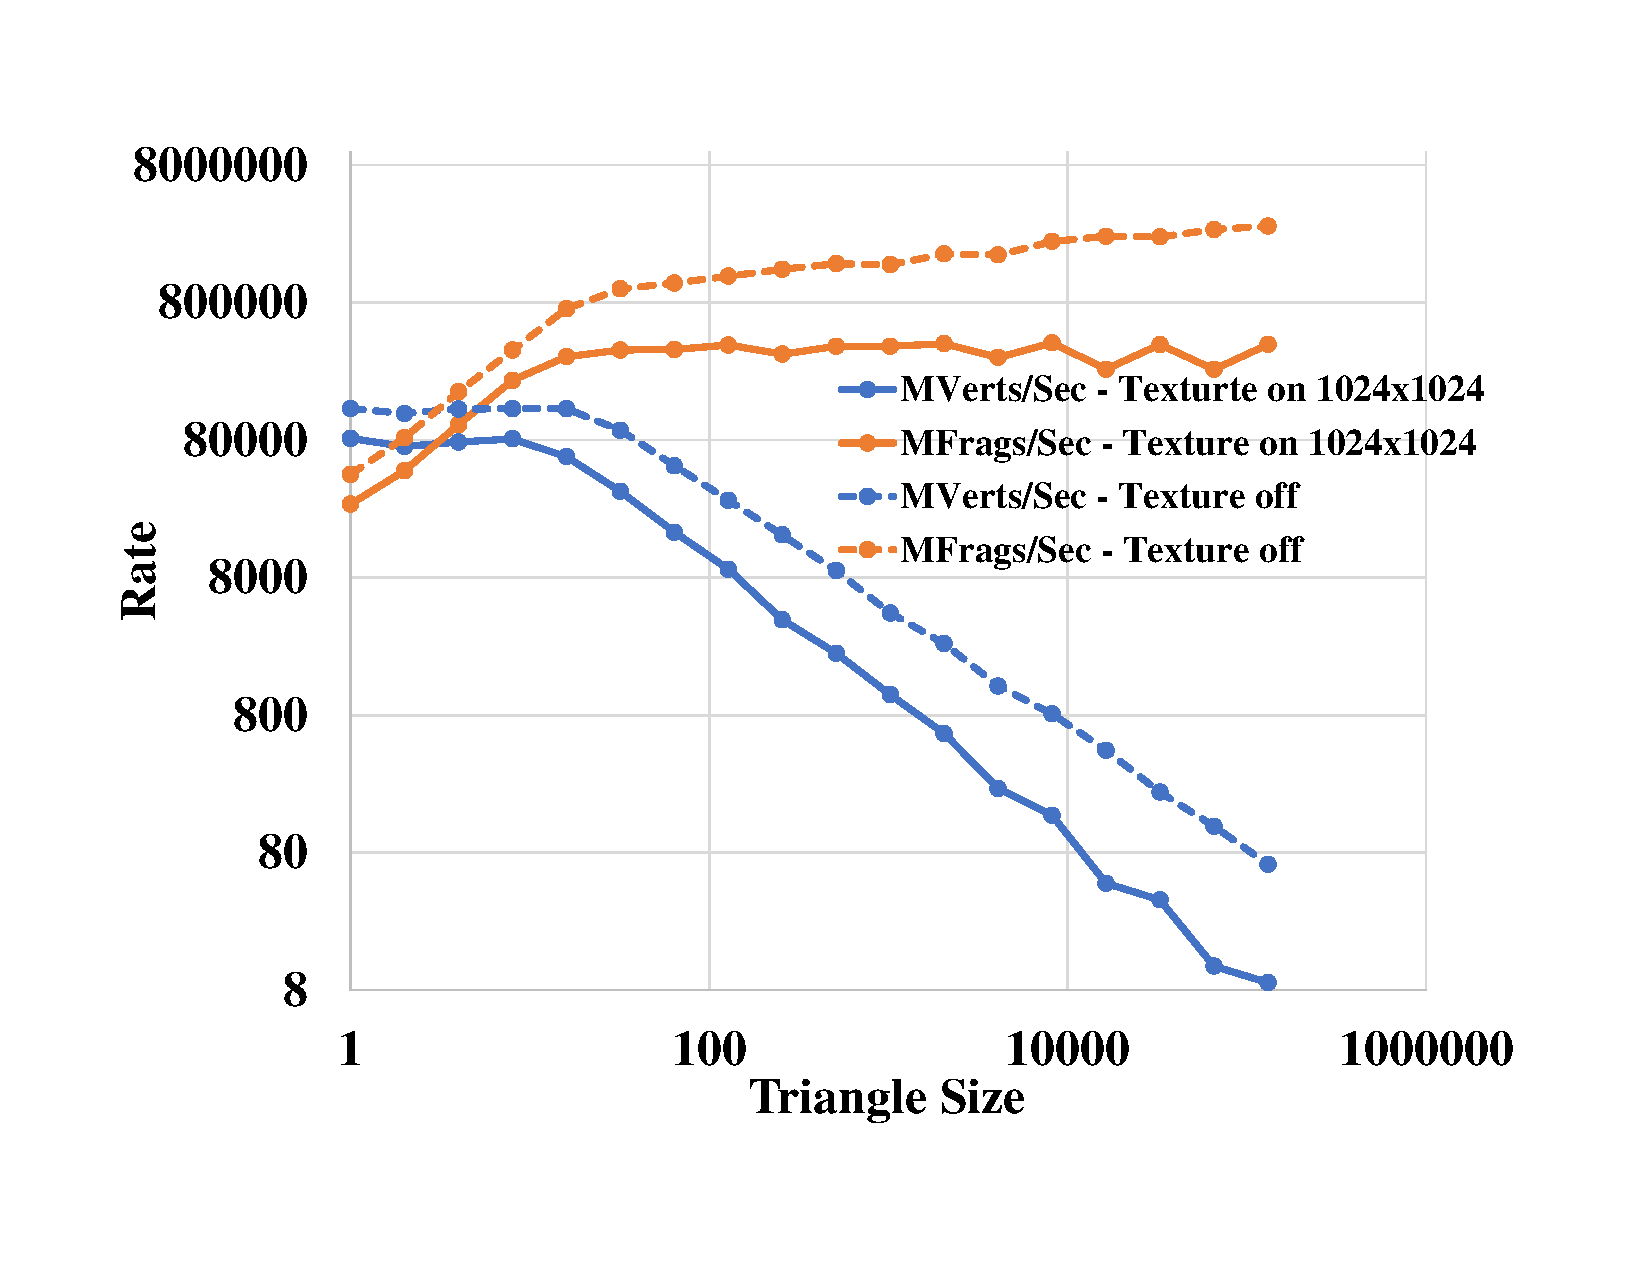
\includegraphics[width=0.49\linewidth]{fig/fill_geo_tx.pdf}}   
 \subfloat[Lit Textured Triangles]
   {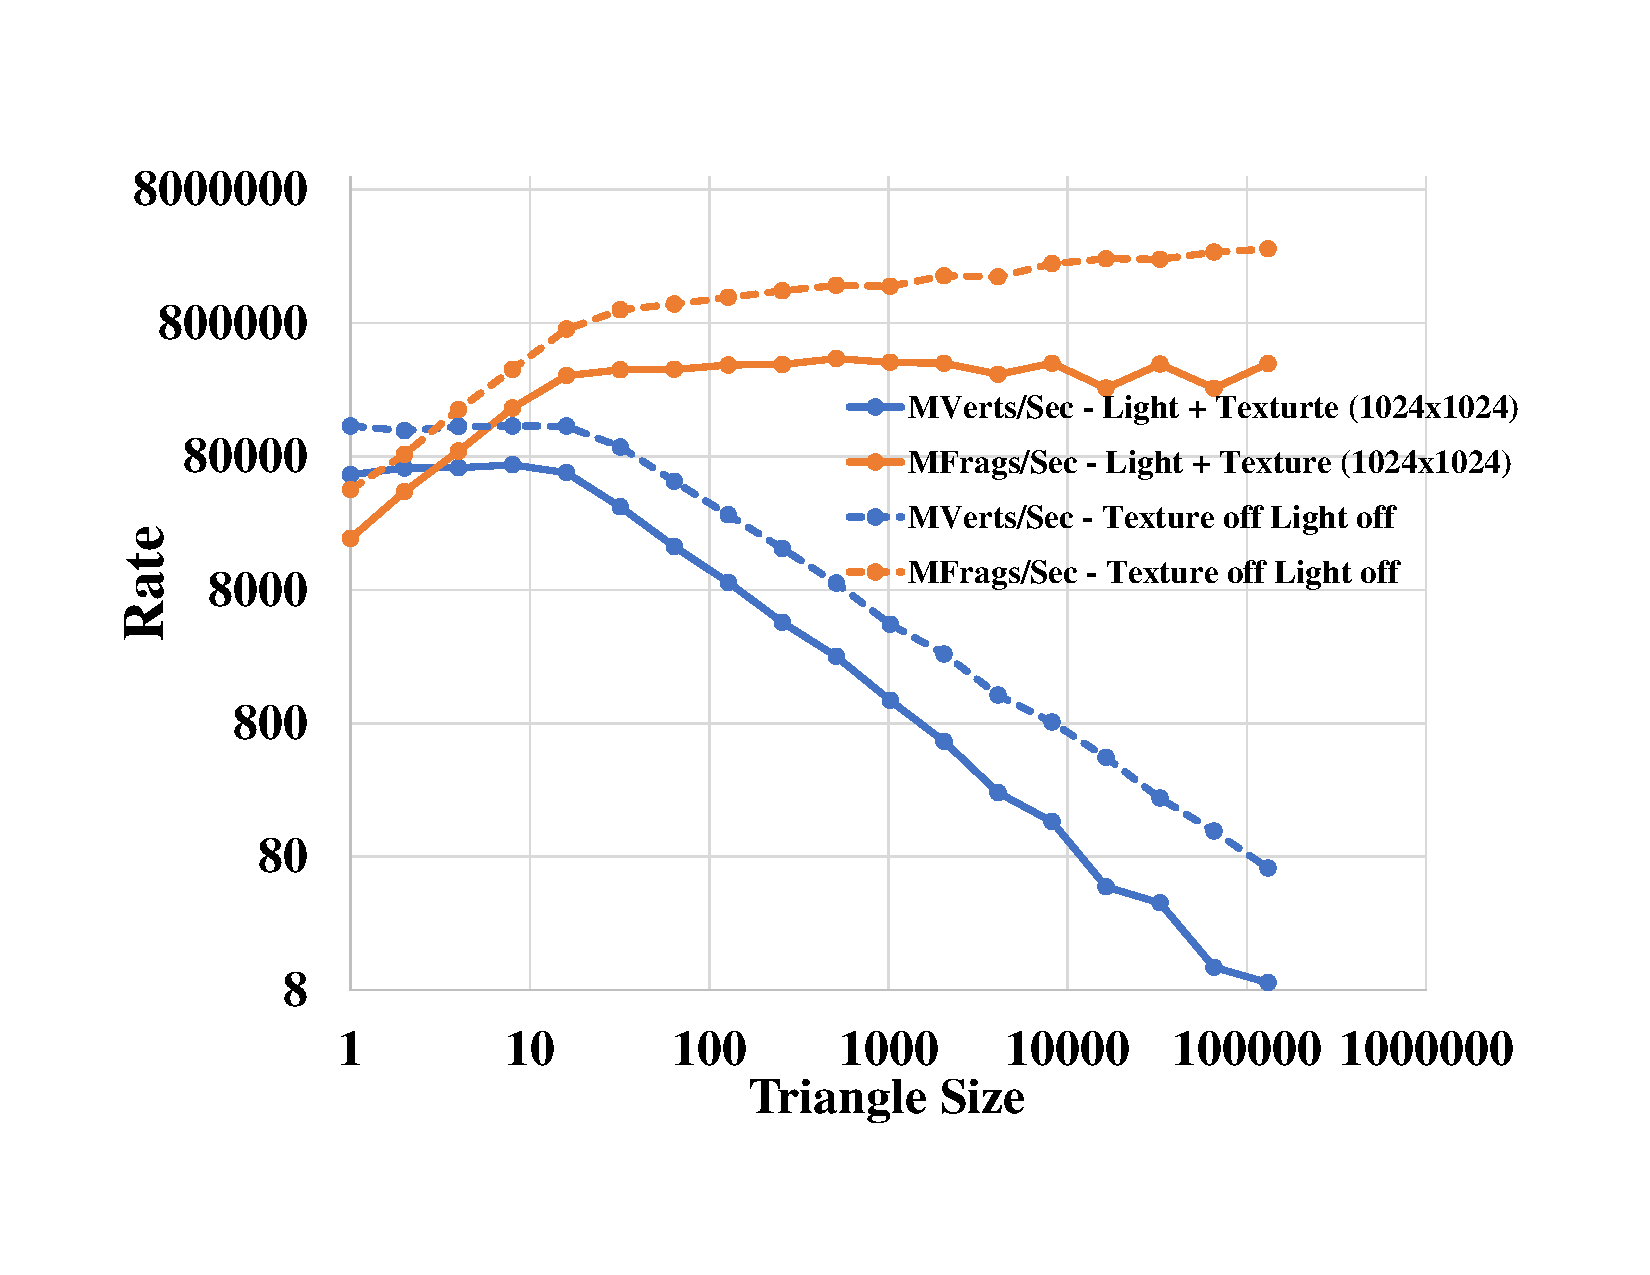
\includegraphics[width=0.49\linewidth]{fig/fill_geo_lit_tx.pdf}}
  \caption{millions of vertices and millions of fragments }
   \label{fig:fill_geo2}
\end{figure} 

%=========================Textured Triangles ===================================%
\subsection{Geometry Rate Vs. Fill Rate on Textured Triangles:}
Now we turn on testing the textured triangles. Following the same methodology as in Section \ref{sec:lit}, we add textures to the triangles of size $1024\times1024$ and vary the triangle size and record the fill and geometry. We tested first with texture of smaller size ($128\times128$), but the graph we got was identical to the untextured one, so we discarded. We assume that this happened due to minimal workload required with small texture size. 

Figure \ref{fig:fill_geo2}(a), compare the fill and geometry rate for textured and untextured triangles. The crossover point is almost the same. Having the same crossover point for the three different scenario tested so far suggests that the graphics card is optimized to have always such a crossover points. The graph also shows an decline in the performance in the textured triangles for both the geometry and fill rate. For the geometry stage, the decline in the number of vertices processed per second is due to the necessary transformation done per vertex (applying the \emph{projector function}\cite{akenine2008real}). The graph in Figure \ref{fig:fill_geo1}(b) and in \ref{fig:fill_geo2}(a) suggest that per-vertex-operation for the lighting is much cheaper for per-vertex-operation for texture which is indicated by the absolute value of geometry rate at certain triangle size. Additionally, the graph shows a divergence in the geometry rate between the textured and untextured. At first glance, this was surprising and we expected a similar behavior as in lit triangles. As the number of triangles decreased with size increases, then less number of vertices needed to be processed. However, we think that this divergence could be due to caching. Since we are using a relatively large texture ($1024\times1024$) and for a big triangles we would required fetching different parts of the texture image that may not be fetched all together into the cache (less spatial locality). 

For rasterization stage, the fill rate decline since the texture operation is more expensive on fragments. During the rasterization, the \emph{corresponder function} (matrix transformation) is applied per fragment and texture value per fragment is interpolated \cite{akenine2008real}. Both could be the reason for the decline in the fill rate. We notice the same divergence happens in fill rate. We assume this is because the geometry stage does not send enough work for the ratserization as the triangle size increase. 

%========================= Lit Texture Triangles====================================%
\subsection{Geometry Rate Vs. Fill Rate on Lit, Textured Triangles:}
Here we use lit, textured triangles and compare the same performance metrics with the unlit, untextured triangles. Figure \ref{fig:fill_geo2}(b) shows that the crossover point did not change which confirm our hypothesis; that the graphics card is optimized for this value. For large triangles (size $\geq 32$) the lighting does not have any impact on both the geometry or the fill rates, then the decline in the performance is purely due to the texture processing. For smaller triangle size, both lighting and texturing contribute in declining

